% !TeX root = ../dissertation.tex
\section{Design}
\label{sec_design}
\label{sec:trillium_design}

\Trillium exports an abstract virtual device and a para-virtual guest driver,
which we use to interpose and forward the OpenCL and CUDA APIs to the host.
Unlike SVGA, which requires translation
layers to ensure that all graphics frameworks APIs can be mapped to the SVGA protocol,
Trillium forwards the lowest layer in the GNU/Linux Graphics stack: the pipe-driver,
effectively remoting OpenCL/CUDA API calls in the guest to the OpenCL/CUDA library in the host.

%\Trillium is composed of a virtual GPU device, and a para-virtual guest driver
%which we use to interpose and forward a GPGPU API through the virtual
%device implementation to the host. Unlike SVGA, which requires translation
%layers to map graphics APIs to the SVGA protocol, Trillium forwards
%Mesa3D pipe-driver functions directly, effectively remoting an OpenCL API
%implementation in the Mesa stack to an OpenCL implementation in the host.

%% \item The historical approach of translating/tunneling other graphics APIs
%% 	over the SVGA protocol is unnecessary, and the protocol can simply be
%% 	extended directly with GPGPU APIs without compromising
%% 	other important properties of the design.

% \Trillium is heavily influenced by the SVGA design, but
Our experience implementing the required TGSI vISA support in the Mesa
graphics stack led us to believe that the TGSI layer is unnecessary.
Not only does this translation introduce additional complexity in the guest
stack, it also hurts performance, as we demonstrate in Section~\ref{sec:eval}.
The guest OpenCL compiler cannot target the native GPU architecture,
and semantic information is lost to the host compiler.
% Because SVGA's native ISA is TGSI, supporting GPGPU workloads in SVGA requires
% GPU code to be expressed in TGSI, rather than in the ISAs produced
% by vendor-specific runtimes (e.g. CUDA's \texttt{PTX} and
% \texttt{SASS}, or AMD's \texttt{SPIR}).
Further, while incorporating a TGSI compiler is possible in open frameworks like OpenCL,
the task is significantly more daunting for closed frameworks like CUDA.
Attempts to translate between TGSI and NVIDIA SASS in the reverse-engineered Nouveau driver
understandably results in code that is significantly less performant
than that produced by the proprietary stack.

\Trillium takes a different approach:
% rather than build a compiler for guest to a virtual ISA which must then be translated in the hypervisor,
% of the production compiler for the actual physical device and
\Trillium forwards API calls for compiling OpenCL code to the hypervisor.
The OpenCL compiler in the host OpenCL framework
(optimized for the physical hardware by the hardware vendor)
is invoked on the forwarded OpenCL code to lower it directly to the physical device ISA.
% If the host OpenCL driver does not support a compiler, \Trillium uses LLVM IR as the virtual ISA.

%\begin{figure}[!th]
%	\centering
%	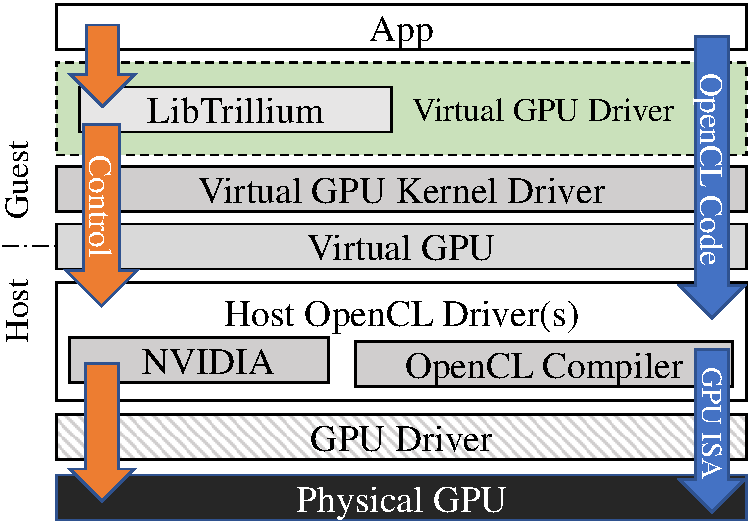
\includegraphics[width=.8\linewidth,trim={0 0 0 0},clip]{images/design/trillium_design.pdf}
%	\caption{{\footnotesize The design of \Trillium.
%            \cjr{FIXME: get designs in position as discussed with Hangchen. }}}
%	\label{fig_trillium} \end{figure}

Figure~\ref{fig_trillium} shows the Trillium design layers in a
generic hypervisor stack. The OpenCL API is forwarded from the
driver similar to the SVGA model.  The OpenCL compute kernel (to be
run on the GPU), can be passed through to the host via hypercalls in
the driver, without being translated to any vISA, where it will
be translated and optimized for the physical GPU in a virtual appliance (Dom~2 in Figure~\ref{fig_trillium}).

\Trillium does not currently guarantee performance isolation and relies on the hardware scheduler.
% task is handed to the hardware.
Performance isolation can easily be implemented via a rate-limiting API scheduler in the
hypervisor, such as in GPUvm~\cite{GPUvm}.

%% \aak{Chris, what level of detail do you want to go to? I'm keeping it minimal
%% here so as to not risk de-anonymizing you. Mentioning that you built this model
%% at VMware will bring questions of why we didn't measure that system instead.}

% \begin{figure}[!th]
% 	\centering
% 	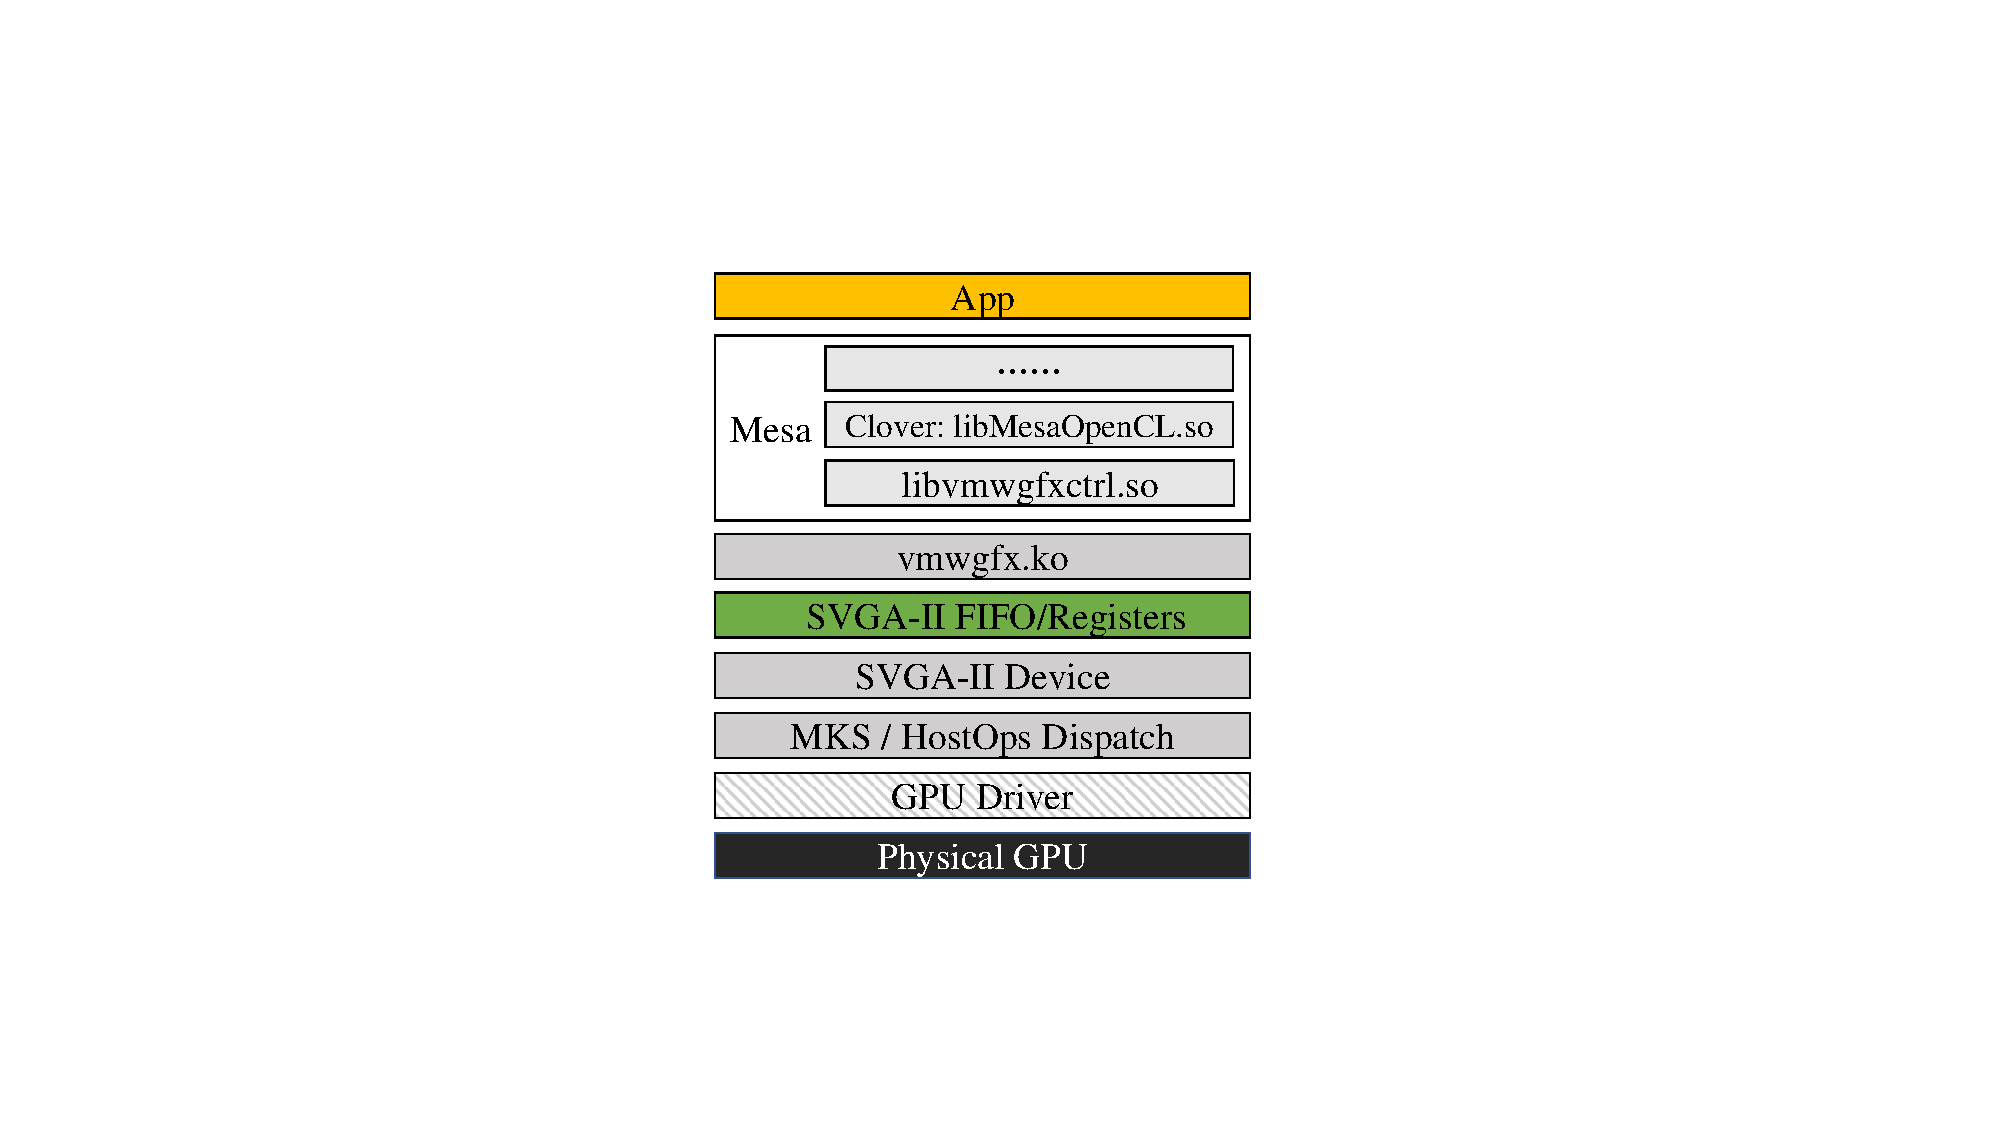
\includegraphics[width=\linewidth,trim={9cm 4cm 9cm 4.5cm},clip]{images/trillium/trillium_classic_single_node.pdf}
% 	\caption{{\footnotesize The design of Trillium Classic.}}
% 	\label{fig_trillium_classic2} \end{figure}


% \subsection{Impact of GPU virtual ISAs}


% % \begin{table}[!th]
% % 	\centering
% % 	\begin{tabular}{l|l|l|l|l|}
% % 		\cline{2-5}
% % 		& Init & MemCpy & Kernel & Total \\ \hline
% % 		\multicolumn{1}{|l|}{ocl+mesa} & \multicolumn{1}{r|}{5.4x} & \multicolumn{1}{r|}{6x} & \multicolumn{1}{r|}{14.5x} & \multicolumn{1}{r|}{7x} \\ \hline
% % 	\end{tabular}
% % 	\caption{Slowdown of Clover OpenCL runtime.}
% % 	\label{tb_clover_slowdown}
% % \end{table}

% The design trades off compatibility: the goal of the virtual TGSI ISA
% for the virtual GPU is to function as universal IR, so that a guest
% compiler is able to produce code that can always be finalized below
% the virtualization layer to a native ISA for the physical GPU. While
% conceptually attractive, the design decision is only effective if
% components elsewhere in the stack (GPU runtimes, compilers, drivers,
% etc.) actually standardize on it.  At present, NVIDIA and AMD GPGPU
% stacks both suppport virtual and native ISAs, but \emph{different}
% ones, neither of which is TGSI, making TGSI effectively an additional
% layer of virtualization on the ISA. We also observe that because both
% AMD and NVIDIA compilers are built on LLVM, there is an opportunity
% for standardizing on LLVM IR as the common IR, which would naturally
% recover the compatibility ceded by the \Trillium design.
